% Methodology section

\subsection{Opetopes}
Originally developed by Baez and Dolan \citep{baez1997higher}, opetopes are mathematical objects that were introduced to weak n-Categories. They are higher-dimensional generalizations of simplicial complexes, capturing directed higher-order interactions with explicit compositional structure. There are multiple ways to define opetopes, but the most common approach is to define them recursively by their boundaries, which are themselves opetopes of lower dimensions. A more traditional way is to define opetopes is using another algebraic structure called operads, which are used to model algebraic structures with multiple operations. Opetopes are a generalization of operads, and they can be used to model higher-dimensional structures with multiple operations. Hence opetopes comes from the word "operation" and "polytope".

We will first look at the more traditional definition of opetopes using operads, and then we will look at the more modern definition of opetopes using boundaries.

\subsubsection{Operads}

Operads are algebraic structures that generalize monoids, groups, and other algebraic structures. Operads consists of:

\begin{itemize}
  \item A collection of operations of different arities.
  \item A notion of composition of these operations.
  \item The composition operations obey certain conditions - associativity and unitality.
\end{itemize}

\textbf{Formal Definition}
\\

Consider a set $\mathbb{X}$, and an integer $n \in \mathbb{N}$.

Now consider a set of functions, lets call it $\mathbb{P}$, where each function $f$ has the signature $\mathbb{X}^n \to \mathbb{X}$:

\begin{equation}
  \mathbb{P}(n) = \{f: \mathbb{X}^n \to \mathbb{X}\}
\end{equation}

where $\mathbb{X}^n$ is the cartesian product of $\mathbb{X}$ with itself $n$ times, i.e.

\begin{equation}
  \mathbb{X}^n = \mathbb{X} \times \mathbb{X} \times \ldots \times \mathbb{X}
\end{equation}

i.e. all of these functions $f$ take in $n$ arguments from $\mathbb{X}$ and return a single element from $\mathbb{X}$.

\begin{figure}[h]
\centering
    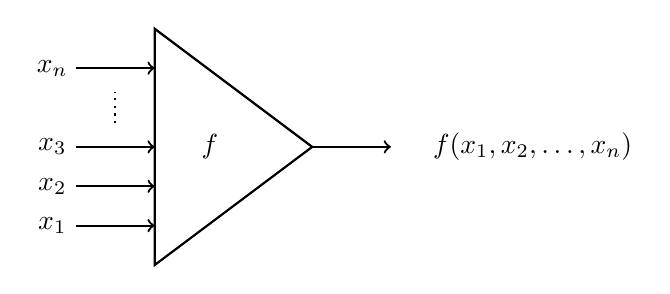
\begin{tikzpicture}
        % Draw the triangle with vertical left edge
        \draw[thick, fill=white] (0,0) -- (0,3) -- (2,1.5) -- cycle;

        % Draw input arrows
        \draw[->, thick] (-1,0.5) -- (0,0.5);
        \draw[->, thick] (-1,1) -- (0,1);
        \draw[->, thick] (-1,1.5) -- (0,1.5);
        \draw[dotted, thick] (-0.5,1.8) -- (-0.5,2.2);
        \draw[->, thick] (-1,2.5) -- (0,2.5);

        % Draw output arrow
        \draw[->, thick] (2,1.5) -- (3,1.5);

        % Add labels
        \node at (0.7,1.5) {$f$};
        \node at (-1.3,0.5) {$x_1$};
        \node at (-1.3,1) {$x_2$};
        \node at (-1.3,1.5) {$x_3$};
        \node at (4.8,1.5) {$f(x_1,x_2,\ldots,x_n)$};
        \node at (-1.3,2.5) {$x_n$};
    \end{tikzpicture}
\end{figure}

If we have a bunch of these sets of functions $\mathbb{P}(k_i)$ for each $k_i \in \mathbb{N}$, then we can define a composition operation $\circ$ on these functions as follows:

Let $f_i \in \mathbb{P}(k_i)$ be a function that takes in $k_i$ arguments from $\mathbb{X}$ and returns a single element from $\mathbb{X}$.

\begin{equation}
    \mathbb{P}(n) \times ( \mathbb{P}(k_1) \times \mathbb{P}(k_2) \times \ldots \times \mathbb{P}(k_n) ) \to \mathbb{P}(k_1 + k_2 + \ldots + k_n)
\end{equation}

\begin{equation}
    f, (f_1, f_2, \ldots, f_n) \mapsto f \circ (f_1, f_2, \ldots, f_n)
\end{equation}

where $f \circ (f_1, f_2, \ldots, f_n) \in \mathbb{P}(k_1 + k_2 + \ldots + k_n)$ is defined as the following diagram:

\begin{figure}[h]
\centering
\begin{tikzpicture}[scale=0.9]
    % Main operation triangle
    \draw[thick, fill=white] (0,0) -- (0,5.5) -- (4,2.75) -- cycle;
    \node at (1.5,2.75) {$f$};

    % First sub-operation triangle
    \draw[thick, fill=white] (-5,0) -- (-5,1.5) -- (-3,0.75) -- cycle;
    \node at (-4.3,0.75) {$f_1$};

    % Second sub-operation triangle
    \draw[thick, fill=white] (-5,2) -- (-5,3.5) -- (-3,2.75) -- cycle;
    \node at (-4.3,2.75) {$f_2$};

    % Third sub-operation triangle (with dotted line indicating more)
    \draw[thick, fill=white] (-5,4) -- (-5,5.5) -- (-3,4.75) -- cycle;
    \node at (-4.3,4.75) {$f_n$};

    % Dotted line between second and third triangles
    \draw[dotted, thick] (-4,3.7) -- (-4,4);

    % Input arrows for first sub-operation
    \draw[->, thick] (-7,0.25) -- (-5,0.25);
    \draw[->, thick] (-7,0.75) -- (-5,0.75);
    \draw[->, thick] (-7,1.25) -- (-5,1.25);
    \node at (-8.4,0.25) {$x_1}$};
    \node at (-8.4,0.75) {$\ldots$};
    \node at (-8.4,1.25) {$x_{k_1}$};

    % Input arrows for second sub-operation
    \draw[->, thick] (-7,2.25) -- (-5,2.25);
    \draw[->, thick] (-7,2.75) -- (-5,2.75);
    \draw[->, thick] (-7,3.25) -- (-5,3.25);
    \node at (-8.4,2.25) {$x_{k_1+1}}$};
    \node at (-8.4,2.75) {$\ldots$};
    \node at (-8.4,3.25) {$x_{k_1+k_2}$};

    % Input arrows for third sub-operation
    \draw[->, thick] (-7,4.25) -- (-5,4.25);
    \draw[->, thick] (-7,4.75) -- (-5,4.75);
    \draw[->, thick] (-7,5.25) -- (-5,5.25);
    \node at (-8.4,4.25) {$x_{k_1+...+k_{n-1}+1}$};
    \node at (-8.4,4.75) {$\ldots$};
    \node at (-8.4,5.25) {$x_{k_1+...+k_{n-1}+k_n}$};

    % Connecting arrows from sub-operations to main operation
    \draw[->, thick] (-3,0.75) -- (0,0.75);
    \draw[->, thick] (-3,2.75) -- (0,2.75);
    \draw[->, thick] (-3,4.75) -- (0,4.75);

    % Output arrow
    \draw[->, thick] (4,2.75) -- (6,2.75);

    % Final output label
    \node at (6,3.5) {$f \circ (f_1, f_2, \ldots, f_n)$};

    % Dotted lines to indicate more inputs for each sub-operation
    \draw[dotted, thick] (-6,1) -- (-6,1.1);
    \draw[dotted, thick] (-6,3) -- (-6,3.1);
    \draw[dotted, thick] (-6,4.5) -- (-6,4.6);

\end{tikzpicture}
\caption{Operadic composition showing how multiple operations $f_1, f_2, \ldots, f_n$ with arities $k_1, k_2, \ldots, k_n$ can be composed with an operation $f$ of arity $n$ to form a new operation of arity $k_1 + k_2 + \ldots + k_n$.}
\label{fig:operadic-composition}
\end{figure}

Associativity of this composition operation works as follows:

\begin{figure}[h]
\centering
    \begin{tikzpicture}[grow'=up]
        \begin{scope}[xshift=-5cm]
            \node {(ab)c}
            child {
                node {ab}
                child {
                    node {a}
                }
                child {
                    node {b}
                }
            }
            child{
                node {c}
            };
        \end{scope}
        \begin{scope}[xshift=0cm]
            \node {(ab)c}
            child{
                node {a}
            }
            child {
                node {bc}
                    child {
                node {b}
                }
                child {
                    node {c}
                }
            };
        \end{scope}
        \begin{scope}[xshift=5cm]
            \node {abc}
            child{
                node {a}
            }
            child {
                node {b}
            }
            child {
                node {c}
            };
        \end{scope}
    \end{tikzpicture}
    \caption{Associativity of operadic composition of arity 3}
\end{figure}

\begin{figure}[h]
\centering
\begin{tikzpicture}[grow'=up, level distance=1.5cm, sibling distance=2cm]
    % First tree: ((ab)c)d
    \begin{scope}[xshift=-10cm]
        \node {((ab)c)d}
        child {
            node {(ab)c}
            child {
                node {ab}
                child {
                    node {a}
                }
                child {
                    node {b}
                }
            }
            child {
                node {c}
            }
        }
        child {
            node {d}
        };
    \end{scope}

    % Second tree: (a(bc))d
    \begin{scope}[xshift=-5cm]
        \node {(a(bc))d}
        child {
            node {a(bc)}
            child {
                node {a}
            }
            child {
                node {bc}
                child {
                    node {b}
                }
                child {
                    node {c}
                }
            }
        }
        child {
            node {d}
        };
    \end{scope}

    % Third tree: (ab)(cd)
    \begin{scope}[yshift=6cm, xshift=0cm]
        \node {(ab)(cd)}
        child {
            node {ab}
            child {
                node {a}
            }
            child {
                node {b}
            }
        }
        child {
            node {cd}
            child {
                node {c}
            }
            child {
                node {d}
            }
        };
    \end{scope}

    % Fourth tree: a((bc)d)
    \begin{scope}[yshift=6cm, xshift=-10cm]
        \node {a((bc)d)}
        child {
            node {a}
        }
        child {
            node {(bc)d}
            child {
                node {bc}
                child {
                    node {b}
                }
                child {
                    node {c}
                }
            }
            child {
                node {d}
            }
        };
    \end{scope}

    % Fifth tree: a(b(cd))
    \begin{scope}[yshift=6cm, xshift=-5cm]
        \node {a(b(cd))}
        child {
            node {a}
        }
        child {
            node {b(cd)}
            child {
                node {b}
            }
            child {
                node {cd}
                child {
                    node {c}
                }
                child {
                    node {d}
                }
            }
        };
    \end{scope}

    \begin{scope}
        \node {abcd}
        child {
            node {a}
        }
        child {
            node {b}
        }
        child {
            node {c}
        }
        child {
            node {d}
        };
    \end{scope}

\end{tikzpicture}
\caption{Associativity of operadic composition of arity 4}
\label{fig:arity-4-associativity}
\end{figure}

This compotision operation $\cdot$ satisfies the following properties:

\begin{itemize}
  \item \textbf{Associativity}: For all $f \in \mathbb{P}(n)$, $g \in \mathbb{P}(k_1)$, $h \in \mathbb{P}(k_2)$, and $i \in \mathbb{P}(k_3)$, we have:

  \begin{equation}
    f \circ (g \circ (h, i)) = (f \circ (g, h)) \circ i
  \end{equation}

  \item \textbf{Unitality}: For all $f \in \mathbb{P}(n)$, we have:

  \begin{equation}
    f \circ (\text{id}_{k_1}, \text{id}_{k_2}, \ldots, \text{id}_{k_n}) = f
  \end{equation}

  where $\text{id}_k$ is the identity function on $\mathbb{X}^k$.
\end{itemize}

Symmetry is not required for operads, but it can be added to form symmetric operads. The symmetry condition is:

\begin{equation}
  f \circ (g_1, g_2, \ldots, g_n) = f \circ (g_{\sigma(1)}, g_{\sigma(2)}, \ldots, g_{\sigma(n)})
\end{equation}

% TODO: verify if this is correct
where $\sigma$ is a permutation of the set $\{1, 2, \ldots, n\}$ or $\sigma \in S_n$ and $g_{\sigma(i)}$ is the $i$-th element of the permutation $\sigma$ i.e. the permutation $\sigma$ permutes the elements of the inputs to the operation $f$.
